\appendix
\section{Model Appendix} 
\subsection{Proofs}
\subsubsection*{Proof of Proposition \ref{prop:wagegrowth}} \label{proof:wagegrowth}
The proposition is derived from the first-order conditions of the firm's problem.
\begin{proof}
    Consider the problem from Lemma \ref{lemma_tenure}.
    The FOC for $v'_{k_1}$ yields (denote $\rho_k$ the shadow cost of $PK_k$ and $\omega_k$ the shadow cost of the expectation condition):
    \[\rho_k\beta(1-s_k)(1-p(v'_{k+1}))-\omega_k+\beta n_k(1-s_k)\frac{\partial (1-v(v'_{k+1}))}{\partial v'_{k+1}}E_{y'|y}\frac{\partial J(y',\{n'_k,v'_{y',k}\}_{k\leq K+1})}{\partial n'_{k+1}}=0\]
    To develop this further, I use the FOC for $w_k$:
    \[-n_k + \rho_k u'(w_k)=0 \iff \rho_k=\frac{n_k}{u'(w_k)}\]
    One can similarly develop $\omega_k$ by applying the FOC for $v'_{y',k+1}$:
    \[ \beta Pr_{y'|y}\frac{\partial J(y',\{n'_k,v'_{y',k}\}_{k\leq K+1})}{\partial v'_{y',k+1}}+ Pr_{y'|y} \omega_k=0 \iff \omega_k = - \beta \frac{\partial J(y',\{n'_k,v'_{y',k}\}_{k\leq K+1})}{\partial v'_{y',k+1}} \forall y'\]
    Applying the envelope theorem one can then note that 
    \[- \frac{\partial J(y',\{n'_k,v'_{y',k}\}_{k\leq K+1})}{\partial v'_{y',k+1}} =  \frac{n'_{k+1}}{u'(w'_{k+1})}\]
    Putting all this together, we get
    \[\frac{n_k}{u'(w_k)}\beta(1-s_k)(1-p(v'_{k+1}))-\beta \frac{n'_{k+1}}{u'(w'_{k+1})}+\beta n_k(1-s_k)\frac{\partial (1-v(v'_{k+1}))}{\partial v'_{k+1}}E_{y'|y}\frac{\partial J(y',\{n'_k,v'_{y',k}\}_{k\leq K+1})}{\partial n'_{k+1}}=0\]
    All that is left is to note that $n'_{k+1}=n_k(1-s_k)(1-p(v'_{k+1}))$, divide by the common terms ($\beta n'_{k+1}$) and rearrange.
    \[ \frac{1}{u'(w'_{k+1})} - \frac{1}{u'(w_k)} = \eta(v'_{k+1}) E_{y'|y} \frac{\partial J(y',\{n'_k,v'_{y',k}\})}{\partial n'_{k+1}} \]
\end{proof}
\subsubsection*{Proof of Proposition \ref{prop:targetwage}} \label{proof:targetwage}
\subsubsection*{Proof of Proposition \ref{prop:layoffs}} \label{proof:layoffs}
This is a straightforward application of the FOC with respect to the layoffs.
\begin{proof}
    Consider the case where $s_k>0$. Then
  \[-\beta n_k (1-p(v'_{k+1}))E_{y'|y} \frac{\partial J(y',\{n'_k,v'_{y',k},z'_k\})}{\partial n'_{k+1}} + \beta E_{y'|y} \frac{\partial J(y',\{n'_k,v'_{y',k},z'_k\})}{\partial z'_{k+1}} \frac{\partial z'_{k+1}}{\partial s_k}- \rho_k \beta (U-R(v'_{k+1}))=0\]  
  Note that the FOC with respect to $w_k$ yields $\rho_k = \frac{n_k}{u'(w_k)}$ and divide by $\beta n_k$ to finalize the proof.
\end{proof}

\subsection{Tenure-specific Severance Payments} \label{severance}
I allow the firm to offer tenure-specific severance payments $sev_k$ to its workers. The severance is constant over time and paid perpetually upon firing and before finding a new job. I show that the severance structure involves higher payments for longer tenured workers (if those workers are on a higher promised value). 
\begin{proposition}
\label{severanceprop}
Fix a firm state. Its severance payments for each tenure $k$ are given by
\begin{equation*}
    \begin{split}
    & \frac{u'(b+sev_k)}{u'(w_k)}=1-\frac{\beta sev_k \frac{\partial p(\theta_{sev_k})}{\partial sev_k}}{1-\beta(1-p(\theta_{sev_k}))} \\
    & \theta_{sev_k} = \theta(arg \max_v [(1-p(v))U(sev_k)+p(v)v]) \\
    \end{split}
\end{equation*}
\end{proposition}
\begin{proof}
I start by describing the unemployment value of a worker with severance payment $sev_k$:
\[U(sev_k) = u(b+sev_k) + \beta \max_v[(1-p(\theta_v))U(sev_k)+p(\theta_v)v]\]
Denote the probability of finding a job with severance payment $sev_k$ as $p(\theta_{sev_k})$. The extra value to the unemployed from the severance payment is then given by
\[\frac{\partial U(sev_k)}{\partial sev_k} = u'(b+sev_k) + \beta (1-p(\theta_{sev_k}))U'(sev_k)=\frac{u'(b+sev_k)}{1-\beta(1-p(\theta_{sev_k}))}\]
Then the total benefit to the firm from raising the severance payment is the slackening of the promised-keeping constraint thanks to this rise in the unemployment value:
\[\lambda_k n_k \beta s_k \frac{\partial U(sev_k)}{\partial sev_k} = \frac{n_k}{u'(w_k)}\beta s_k \frac{u'(b+sev_k)}{1-\beta(1-p(\theta_{sev_k}))}\]
On the cost side, the firm internalizes the net present value of the severance payments when firing $n_ks_k$ workers:
\[\frac{\partial}{\partial sev_k}\Big[n_k s_k \beta \frac{sev_k}{1-\beta(1-p(\theta_{sev_k}))}\Big]=n_ks_k\beta \frac{[1-\beta(1-p(\theta_{sev_k}))]-\beta sev_k \frac{\partial p(\theta_{sev_k})}{\partial sev_k}}{[1-\beta(1-p(\theta_{sev_k}))]^2}\]
The optimal severance payment then follows from the first-order condition:
\[ \frac{n_k}{u'(w_k)}\beta s_k \frac{u'(b+sev_k)}{1-\beta(1-p(\theta_{sev_k}))} = n_ks_k\beta \frac{[1-\beta(1-p(\theta_{sev_k}))]-\beta sev_k \frac{\partial p(\theta_{sev_k})}{\partial sev_k}}{[1-\beta(1-p(\theta_{sev_k}))]^2}\]
Rearranging gives the result.
\[\frac{u'(b+sev_k)}{u'(w_k)}=1-\frac{\beta sev_k \frac{\partial p(\theta_{sev_k})}{\partial sev_k}}{1-\beta(1-p(\theta_{sev_k}))}\]
\end{proof}
Note that, besides $u'(w_k)$, all the components of the severance payment are independent of both the firm state and the worker tenure. 
It is immediate to notice then that higher paid workers will have higher severance payments: as $\frac{1}{u'(w_k)}$, the value to the firm of the severance payment goes up, while costs stay the same. Therefore, the firm will optimally choose to offer higher severance payments to higher paid workers. \\
This equation is also easy to implement numerically: using the formulation in Appendix~\ref{dual}, where $\rho_k\equiv u'(w_k)$ is a state variable, I can immediately compute the payments for all the firm states, before solving the rest of the firm problem.
\subsection{Microfounding the Wage Noncontractability} \label{microfoundation}
Consider a simplified, 2-period version of the model. The firm starts with measure $n=2$ of workers, half of them of high quality and the other half of low. I allow the firm to offer quality-contingent wages in whichever way it likes. \\
I show that, under a sufficiently small elasticity of job search probability with respect to promised value $v'$, $\eta(v')\equiv\frac{\partial (1-p(v')) /\partial v'}{(1-p(v'))}$, the firm will optimally choose to keep wages constant across matches of different quality.
\subsection{Recursive Lagrangian Approach} \label{dual}
The original design of the problem would require solving promised values $v'_{y',k}$ for both each tenure step and each future productivity state. Following \textcite{balke2022}, I solve the following Pareto problem:
\begin{equation*}
\begin{split}
\mathcal{P}(y,\{n_k,\rho_k,z_k\}) = &\inf_{\omega_k} \sup_{\tilde{n},\tilde{v},\{w_k,s_k,v'_k\}}  yF(n,z) - \sum_k n_kw_k - \kappa_f - \tilde{n}\frac{c}{q(\theta_{\tilde{v}})}   \\
& + \sum_k\rho_k(u(w_k)+\beta[s_kU+(1-s_k)R(v'_{k+1})] \\
& -\beta\sum_k \omega_k v'_{k+1}+\beta E_{y'|y}\mathcal{P}(y',\{n'_k,\omega_k,z'_k\})    
\end{split}
\end{equation*}

where
\[\mathcal{P}(y,\{n_k,\rho_k,z_k\}) \equiv \sup_{\{v_k\}} J(y,\{n_k,v_k,z_k\})+\sum_k \rho_k v_k \]
The following proof (for $K\rightarrow\infty$ but the proof extends trivially to finite $K$) establishes its equivalence with the initial problem. It follows the steps of \textcite{balke2022}, extending it to the case of a multi-worker firm.
\begin{proof}
We have the following recursive formulation for $J$:
\begin{equation*}
    \begin{split}
 J(y,\{n_k,v_k,z_k\}_{k\leq K}) =
    %Max
    & \max_{\tilde{n},\tilde{v},\{v'_k,v'_{y',k},w_{k},s_{k}\}_{k\leq K}} 
    %Production
    yF(\sum_k n_k,\frac{\sum n_kz_k}{\sum n_k})-
    %Wage
    \sum_k w_kn_k
    %Size
    -\tilde{n}\frac{c}{q(\tilde{v})}-\kappa_f \\
    %Expectation
    & +\beta E_{y'|y} J(y',\{n'_k,v'_k,z'_k\}_{k\leq K+1}) \\
(\lambda_k) \: & u(w_k) + \beta [s_k U + (1-s_k)R(v'_{k+1})=v_k] \; \forall k\leq K \\
(\omega_k)    & v'_{k+1} = E_{y'|y} v'_{k+1,y'} \; \forall k\leq K \\
    & n'_{k+1} = n_k(1-s_k)(1-p(v'_{k+1}))+\tilde{n}\; \forall k\leq K \\
    & z'_{k+1} = min(\frac{z_k}{1-s_k},1)\; \forall k\leq K \\
    & n'_0 = \tilde{n}, v'_0 = \tilde{v}, z'_0 = z_0
    \end{split}
\end{equation*}
Consider the Pareto problem
\[\mathcal{P}(y,\{n_k,\rho_k,z_k\}) = \sup_{\{v_k\}} J(y,\{n_k,v_k,z_k\})+\sum_k \rho_k v_k \]
I first substitute the definition of $J$ together with its constraints into $\mathcal{P}$:
\begin{equation*}
    \begin{split}
 \mathcal{P}(y,\{n_k,\rho_k,z_k\}) =
    %Max
    & \sup_{\tilde{n},\tilde{v},\{v_k,v'_{k},v'_{y',k},w_{k},s_{k}\}_{k\leq K}} 
    %Production
    yF(\sum_k n_k,\frac{\sum n_kz_k}{\sum n_k})-
    %Wage
    \sum_k w_kn_k
    %Size
    -\tilde{n}\frac{c}{q(\tilde{v})}-\kappa_f \\
    %Expectation
    & +\beta E_{y'|y} J(y',\{n'_k,v'_k,z'_k\}_{k\leq K+1}) + \sum_k \rho_k v_k  \\
(\lambda_k) \: & u(w_k) + \beta [s_k U + (1-s_k)R(v'_{k+1})=v_k] \; \forall k\leq K \\
(\omega_k) \:   & v'_{k+1} = E_{y'|y} v'_{k+1,y'} \; \forall k\leq K \\
    & n'_{k+1} = n_k(1-s_k)(1-p(v'_{k+1}))+\tilde{n}\; \forall k\leq K \\
    & z'_{k+1} = min(\frac{z_k}{1-s_k},1)\; \forall k\leq K \\
    & n'_0 = \tilde{n}, v'_0 = \tilde{v}, z'_0 = z_0
    \end{split}
\end{equation*}
I now substitute in the promise-keeping constraint:
\begin{equation*}
    \begin{split}
 \mathcal{P}(y,\{n_k,\rho_k,z_k\}) =
    %Max
    & \sup_{\tilde{n},\tilde{v},\{v'_k,v'_{y',k},w_{k},s_{k}\}_{k\leq K}} 
    %Production
    yF(\sum_k n_k,\frac{\sum n_kz_k}{\sum n_k})-
    %Wage
    \sum_k w_kn_k
    %Size
    -\tilde{n}\frac{c}{q(\tilde{v})}-\kappa_f \\
    %Expectation
    & +\beta E_{y'|y} J(y',\{n'_k,v'_k,z'_k\}_{k\leq K+1}) + \sum_k \rho_k (u(w_k) + \beta [s_k U + (1-s_k)R(v'_{k+1})])  \\
(\omega_k) \:    & v'_{k+1} = E_{y'|y} v'_{k+1,y'} \; \forall k\leq K \\
    & n'_{k+1} = n_k(1-s_k)(1-p(v'_{k+1}))+\tilde{n}\; \forall k\leq K \\
    & z'_{k+1} = min(\frac{z_k}{1-s_k},1)\; \forall k\leq K \\
    & n'_0 = \tilde{n}, v'_0 = \tilde{v}, z'_0 = z_0
    \end{split}
\end{equation*}
I introduce the $\omega_k$-constraints with weights $\beta$ into the problem:
\begin{equation*}
    \begin{split}
 \mathcal{P}(y,\{n_k,\rho_k,z_k\}) =
    %Max
    & \inf_{\{\omega_k\}}\sup_{\tilde{n},\tilde{v},\{v'_k,v'_{y',k},w_{k},s_{k}\}_{k\leq K}} 
    %Production
    yF(\sum_k n_k,\frac{\sum n_kz_k}{\sum n_k})-
    %Wage
    \sum_k w_kn_k
    %Size
    -\tilde{n}\frac{c}{q(\tilde{v})}-\kappa_f \\
    %Expectation
    & +\beta E_{y'|y} J(y',\{n'_k,v'_k,z'_k\}_{k\leq K+1}) + \sum_k \rho_k (u(w_k) + \beta [s_k U + (1-s_k)R(v'_{k+1})])  \\
    & + \sum_k \beta\omega_k(E_{y'|y}v'_{y',k+1}-v'_{k+1})\\
    & n'_{k+1} = n_k(1-s_k)(1-p(v'_{k+1}))+\tilde{n}\; \forall k\leq K \\
    & z'_{k+1} = min(\frac{z_k}{1-s_k},1)\; \forall k\leq K \\
    & n'_0 = \tilde{n}, v'_0 = \tilde{v}, z'_0 = z_0
    \end{split}
\end{equation*}
I then rearrange the value function by moving $E_{y'|y}\sum_k \beta\omega_kn'_{k+1}v'_{y',k+1}$ (additional constraints are dropped to simplify notation):
\begin{equation*}
    \begin{split}
 \mathcal{P}(y,\{n_k,\rho_k,z_k\}) =
    %Max
    & \inf_{\{\omega_k\}}\sup_{\tilde{n},\tilde{v},\{v_k,v'_{y',k},w_{k},s_{k}\}_{k\leq K}} 
    %Production
    yF(\sum_k n_k,\frac{\sum n_kz_k}{\sum n_k})-
    %Wage
    \sum_k w_kn_k
    %Size
    -\tilde{n}\frac{c}{q(\tilde{v})}-\kappa_f \\
    %Expectation
    & +\beta E_{y'|y} [J(y',\{n'_k,v'_k,z'_k\}_{k\leq K+1}) + \sum_k\omega_kv'_{y',k+1}]\\
    & \sum_k \rho_k (u(w_k) + \beta [s_k U + (1-s_k)R(v'_{k+1})])- \sum_k \beta\omega_kv'_{k+1}  
    \end{split}
\end{equation*}
Lastly, I split the sup:
\begin{equation*}
    \begin{split}
    \mathcal{P}(y,\{n_k,\rho_k,z_k\}) =
    %Max
    & \inf_{\{\omega_k\}}\sup_{\tilde{n},\tilde{v},\{v'_k,w_{k},s_{k}\}_{k\leq K}} 
    %Production
    yF(\sum_k n_k,\frac{\sum n_kz_k}{\sum n_k})-
    %Wage
    \sum_k w_kn_k
    %Size
    -\tilde{n}\frac{c}{q(\tilde{v})}-\kappa_f \\
    %Expectation
    & +\beta E_{y'|y} [\sup_{v'_{y',k+1}}J(y',\{n'_k,v'_k,z'_k\}_{k\leq K+1}) + \sum_k\omega_kv'_{y',k+1}]\\
    & \sum_k \rho_k (u(w_k) + \beta [s_k U + (1-s_k)R(v'_{k+1})])- \sum_k \beta\omega_kv'_{k+1}     
    \end{split}
\end{equation*}
From this, one can note that, by definition of $\mathcal{P}$ \[\sup_{v'_{y',k+1}}J(y',\{n'_k,v'_k,z'_k\}_{k\leq K+1}) + \sum_k\omega_kv'_{y',k+1} = \mathcal{P}(y',\{n'_k,\omega_k,z'_k\})\]
We thus arrive to the formulationof the problem as described at the beginning, not involving finding future state-specific promised values $v'_{y',k}$.
\end{proof}
\subsection{Block Recursivity} \label{blocrecur}
I introduce an assumption that would allow for a block recursive eqiulibrium under the same conditions as in \textcite{schaal2017}. Block recursivity requires an indifference condition, either on the side of the firms or on the side of the workers. Under two-sided ex-post heterogeneity, that is not immediately achievable. \\
\textcite{schaal2017} shows that, in a setting similar to mine, but with transferable utility between workers and firms, which he achieves due to the risk-neutral worker utility function, firms all have the same preferences across all the submarkets that they may post vacancies in. 
Define the minimal hiring cost as 
\[k = \min_{v} [v + \frac{c}{q_v}]\]
Due to transferable utility, the cost of employing the worker from submarket $v$ becomes simply the value $v$. Thus, the optimal entry of vacancies in \textcite{schaal2017} can be summarized by 
\[\theta_v [v + \frac{c}{q_v} - k]=0\]
Meaning that either a submarket $v$ minimizes the hiring cost or it is closed. This condition is completely independent of the distribution of firms and workers, exactly because the one component where the firm type might come through, the cost of employing a worker from submarket $v$, is completely independent from the firm's state due to transferable utility.\\
Utility is not transferable in my model, and thus different firms may face different costs of employing a worker at some value $v$ (for example, fixing $y$ and $z$, small firms prefer high values $v$ due to their intention to upsize). To get around that, I split the value $v$ that the worker would get upon getting hired into two components, the sign-on wage $w_v$ and the remaining value $v_0$ such that
\[u(w_v)+\beta v_0= v\]
This additional wage payment is incurred immediately upon hiring, allowing the remaining value that the firm owes to its worker, $v_0$, to be completely independent of the submarket $v$. Essentially, from the firm's perspective, submarkets now differ not in the value that firms would owe to the workers, but in this sign-on wage. The cost minimization problem then becomes 
\[k = \min_{v} [w_v + \frac{c}{q_v}]\]
This problem is now again completely independent of the firm's state, and thus the distribution of firms and workers no longer affects the tightness function $q_v$.\textcite{schaal2017} shows that, in a setting similar to mine, but with transferable utility between workers and firms, which he achieves due to the risk-neutral worker utility function, firms all have the same preferences across all the submarkets that they may post vacancies in. Then setting $\theta_v$ such that 
\newpage
\section{Quantitative Appendix}
% Define colors
\definecolor{state}{RGB}{0,128,0}       % green
\definecolor{ctrl}{RGB}{255,140,0}      % orange
\definecolor{ex}{RGB}{255,0,255}        % magenta
\definecolor{nextstate}{RGB}{0,0,255}    % blue
\definecolor{value}{RGB}{128,128,0}    % yellow

\subsection{Variables}
\subsection*{\textcolor{state}{Endogenous state variables}}
\begin{align*}
&\textcolor{state}{\{n_{k}\}_{k\leq K}}, \textcolor{state}{\{\rho_{k}}, \textcolor{state}{z_{k}\}_{1\leq k\leq K}}
\end{align*}
\textbf{Code:} \texttt{states: size, rho, q}

\subsection*{\textcolor{ex}{Exogenous state variables}}
\begin{align*}
&\textcolor{ex}{y}
\end{align*}
\textbf{Code:} \texttt{z}

\subsection*{\textcolor{ctrl}{Control variables}}
\begin{align*}
&\textcolor{ctrl}{\tilde{n}}, \textcolor{ctrl}{\{\rho'_k\}_{1\leq k\leq K}}, \textcolor{ctrl}{\{s_k\}_{k\leq K}}
\end{align*}
\textbf{Code:} \texttt{hiring, rho\_star, sep\_star}

\subsection*{\textcolor{value}{Value function}}
\begin{align*}
&\textcolor{value}{\mathcal{P}(\textcolor{ex}y,\textcolor{state}{\{n_k,\rho_k,z_k\}})}
\end{align*}
\textbf{Code:} \texttt{ERho\_star, EJ\_star}
\subsection{Equations}
Equations (1)--(21): \textcolor{value}{Value function in olive} (given by value and its gradient guesses from future states), \textcolor{state}{states in }\textcolor{state}{green} (given), \textcolor{ctrl}{controls} in \textcolor{ctrl}{orange} (given by policy guess from current states), next period \textcolor{ex}{exogenous states in magenta} (to be summed over), next period \textcolor{nextstate}{states in blue}, parameters in black.
\begin{align}
%0&=\textcolor{ctrl}{\rho^*_{k+1}}-\textcolor{state}{\rho_k} - \eta(v'_{k+1})E\frac{\partial J(\textcolor{ex}{y'},\textcolor{nextstate}{\{n'_k,v'_{y',k},z'_k\})}}{\partial \textcolor{nextstate}{n'_{k+1}}} \\
0&=\textcolor{ctrl}{\rho'_{k+1}}-\textcolor{state}{\rho_k} - \eta(E \frac{\partial P(\textcolor{ex}{y'},\textcolor{nextstate}{\{n'_k,\rho'_{k},z'_k\})}}{\partial \textcolor{nextstate}{\rho'_{k+1}}})E\frac{\partial \mathcal{P}(\textcolor{ex}{y'},\textcolor{nextstate}{\{n'_k,\rho'_{k},z'_k\})}}{\partial \textcolor{nextstate}{n'_{k+1}}} \\
% ... (rest of equations unchanged for brevity) ...
\end{align}


\section{Data Appendix}
\
\subsection{Wage Growth} \label{wagegrowthK}
I use the same sample to plot the log (real) wage growth across first 30 years of tenure. 
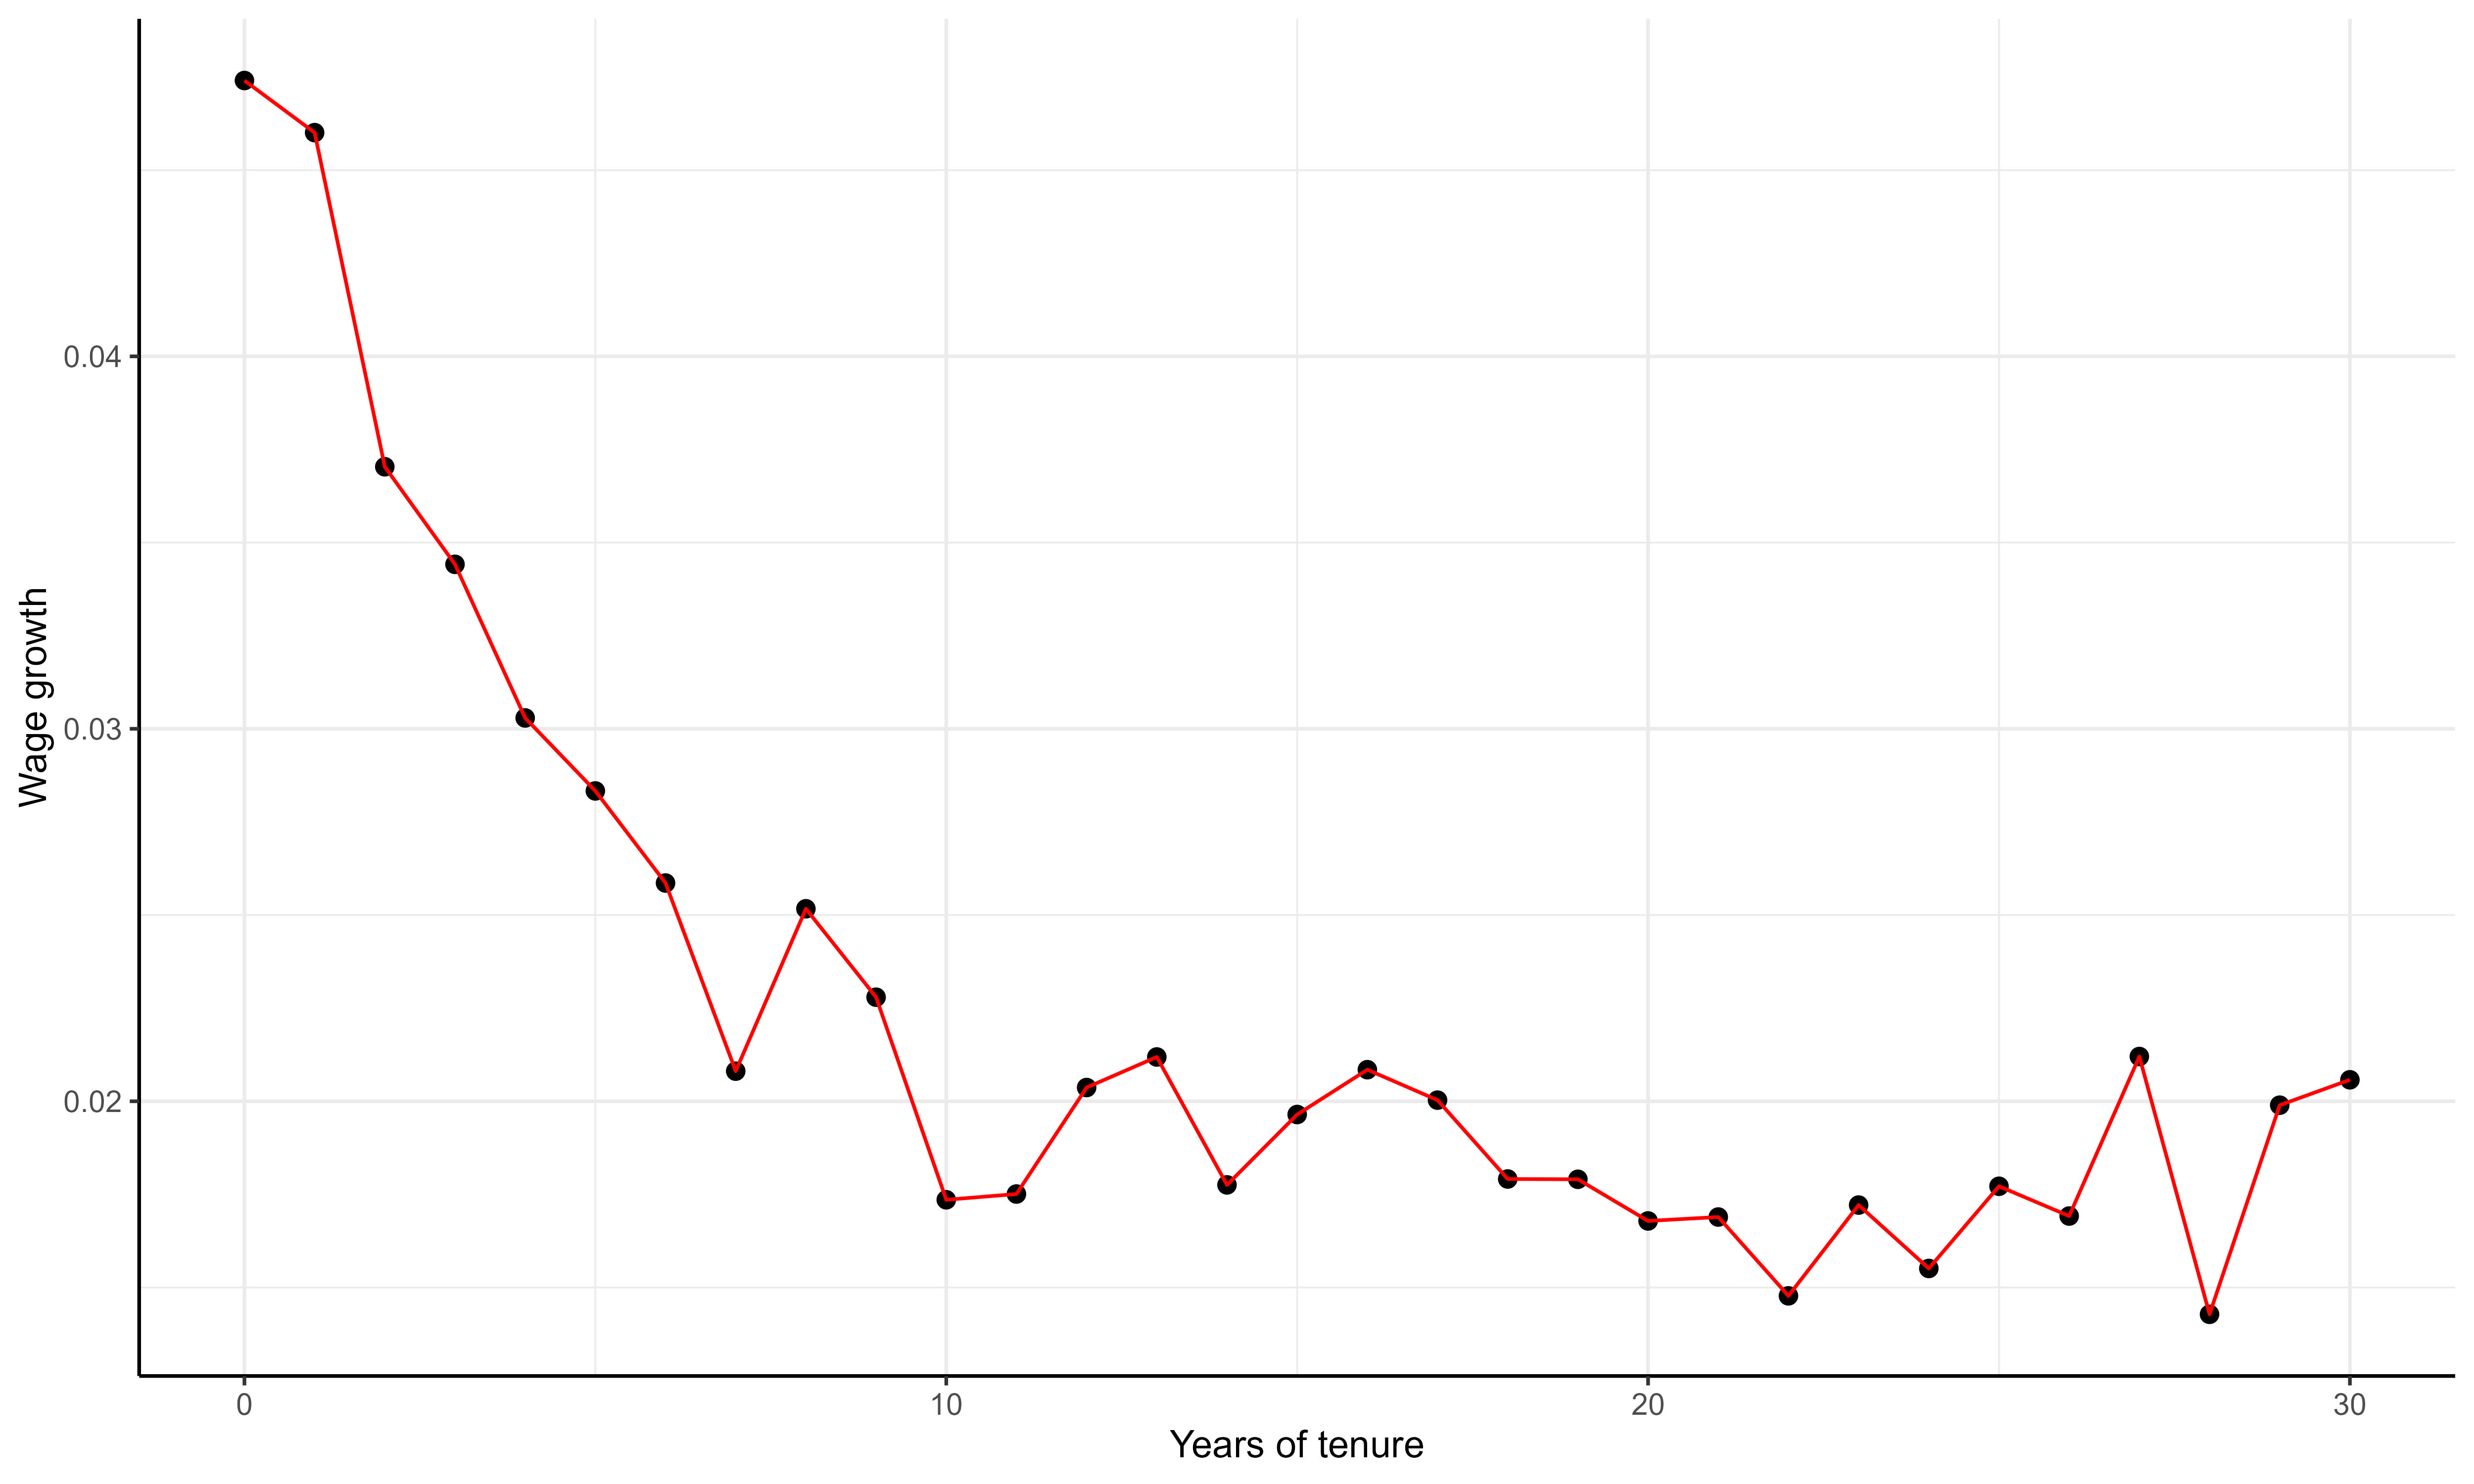
\includegraphics[width=0.75\textwidth]{Wage growth across tenure under 30,cutoff 100.jpg} \\
The wage growth appears to flatten after about 10 years of tenure, suggesting that it is not quantitatively costly to use $K=10$ as an approximation of the firm problem from Definition \ref{firmproblem}.

